\chapter{Sequence Automaton}
\label{chap-sequence-automaton}
\index{Sequence Automaton}
%The construction of local grammars can be a long process in which Unitex users may have to make several additions or modifications.


The construction of local grammars can be a long process during which the linguist repeated many times the same operations. The aim of the Seq2Grf program is to produce quickly and automatically local grammars.


\bigskip
\noindent This program can be used in command line mode or by clicking on "Construct Sequences Automaton" in the Text Menu.
The use of the command Seq2Grf is described in section~\ref{Seq2Grf}.

\bigskip
\noindent For a given document (TEILite or txt format files or SNT when preprocessed for this task with {STOP} tags) this programs builds a single automaton that recognizes all the sequences contained in the document.

\bigskip
\noindent Special attention should be paid to the establishment of the list of sequences that are recognized by the graph.

\bigskip
\noindent This chapter presents the file formats supported by the Seq2Grf program, the construction of the sequence automaton, and the use of wildcards.
\bigskip


\section{Sequences Corpus}
We call sequences corpus or qualified corpus a list of sequences of one or several words that we want to be recognized by only one local grammar graph. 
\bigskip

This sequences corpus is stored in one single file wich must be from one of the following formats :
\begin{itemize}
	\item raw text files in which sequences are delimited by end of line 
	\item SNT files already processed with this menu : sequences will be delimited by the {STOP} tag.
	\item TEILite files in which sequences are delimited by the following xml tag :	
		\begin{verbatim}<seg type="sequence">example</seg>
		\end{verbatim}
\end{itemize}
\pagebreak 
\indent Since the corpus contains specific sequences, it must be done by hand. This means that you have to either write all the sequences in a raw text file and separate them by an end  of line (figure~\ref{fig8-1CorpusTxt}), or insert the specific xml tag in an existing TEILite Document (figure~\ref{fig8-3CorpusTEI}). The preprocessing of TXT or XML Documents will produce a SNT file that is used for the build of the Sequence Automaton (figure~\ref{fig8-2CorpusSNT}). This File can be used as an input. The produced graph will only recognize the sequences that are correctly delimited. Production of local grammars is automatic only from a corpus of well-defined sequences. If you have such a corpus, then the time saved is considerable.

\begin{figure}[!ht]
	\begin{minipage}[h!]{0.5\linewidth}
		\centering
		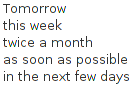
\includegraphics[scale=0.6]{resources/img/fig8-1tomorrow.png}	
		\caption{TXT\label{fig8-1CorpusTxt}}
		\label{fig7-TXT}
	\end{minipage}
	\hspace{0.1cm}
	\begin{minipage}[h!]{0.5\linewidth}
		\centering
		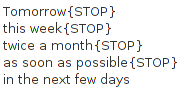
\includegraphics[scale=0.6]{resources/img/fig8-2tomorrowSNT.png}
		\caption{SNT\label{fig8-2CorpusSNT}}
	\end{minipage}
	\hspace{0.1cm}
\end{figure}
\begin{figure}[!ht]
	\begin{minipage}[h!]{\linewidth}
		\centering
			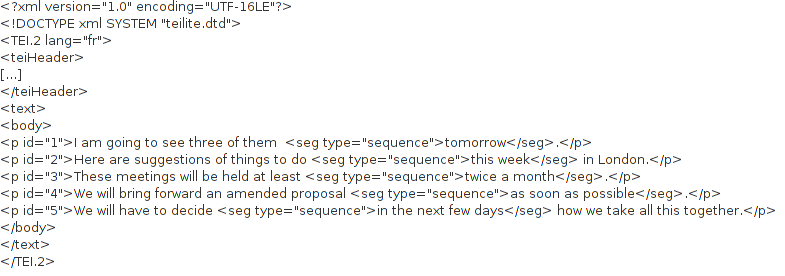
\includegraphics[width=14cm]{resources/img/fig8-3tomorrowTEI.png}
			\caption{TEILite\label{fig8-3CorpusTEI}}
	\end{minipage}
\end{figure}
%%%%%%%%%%%%%%%%%%%%%%%%%%%%%%%%%%%%%%%%%%%%%%%%%%%%%%%%%%%%%%%%%%%
\section{Usage}
In order to create a sequence automaton, click on "Construct Sequence Automaton" in the "Text" menu. You will then see the window coming up as in figure~\ref{fig8-4Menu1}.

This window will allow you to set the parameters to produce a sequence automaton.
You have to follow these three steps :
\begin{itemize}
\item choose the sequence corpus : that can be a file which format is one of the three described in the previous section. The file format
is automatically detected according to the file extension. 


\item set the specific options :
Applying the beautifying algorithm will place each box so that the resulting graph is smaller and as easily readable as possible.
The exact case matching will put litteral tokens into braces in the graph so that the graph doesn't match tokens with same letters but with case differences.

You can set more options to produce a graph that allow approximate matching :
you can set the number of jokers to be used to produce new sequences derived from the sequences of the original corpus, and what kind of joker can be used.
All the details about the use of jokers is detailed in section \ref{approximation}

\item choose the directory where the graph will be saved.
\end{itemize}
\medskip
\begin{figure}[h!]
	\begin{minipage}[h!]{0.5\linewidth}	
		\centering
			%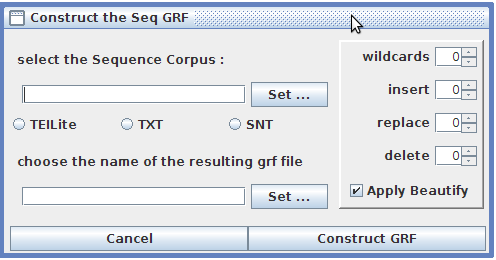
\includegraphics[width=8cm]{resources/img/fig8-0seq2grf1.png}
			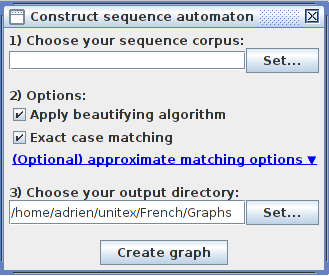
\includegraphics[width=8cm]{resources/img/fig8-4Menu1.png}
			\caption{The sequence automaton menu\label{fig8-4Menu1}}
	\end{minipage}	
	\hspace{0.3cm}
	\begin{minipage}[h!]{0.5\linewidth}	
		\centering
			%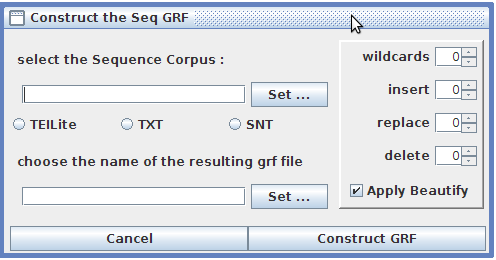
\includegraphics[width=8cm]{resources/img/fig8-0seq2grf1.png}
			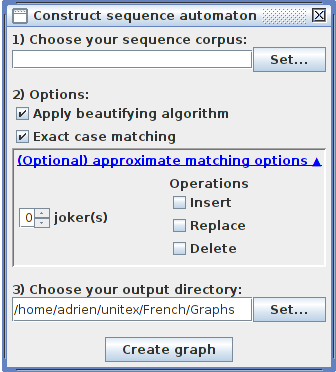
\includegraphics[width=8cm]{resources/img/fig8-4Menu2.png}
			\caption{Options of the sequence automaton menu\label{fig8-4Menu2}}
	\end{minipage}
\end{figure}

\bigskip
\noindent You can see in figures~\ref{fig8-5GRFnoBeautify} and~\ref{fig8-6GRFBeautify} the graphes without wildcards produced without or with beautify.


\begin{figure}[!ht]
	\begin{minipage}[h!]{0.5\linewidth}
		\centering
		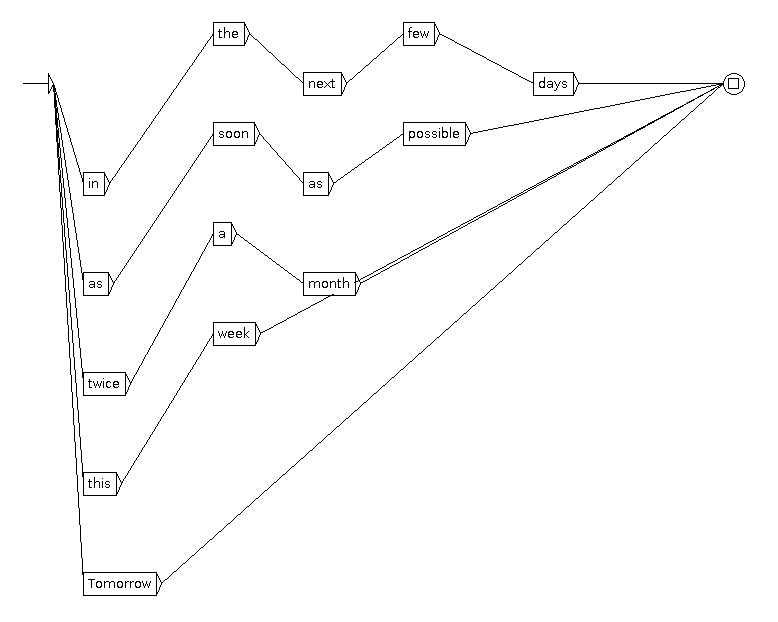
\includegraphics[width=8cm]{resources/img/fig8-5GRFnoBeautify.png}	
		\caption{Automaton without beautify option\label{fig8-5GRFnoBeautify}}
	\end{minipage}
	\hspace{0.1cm}
	\begin{minipage}[h!]{0.5\linewidth}
		\centering
		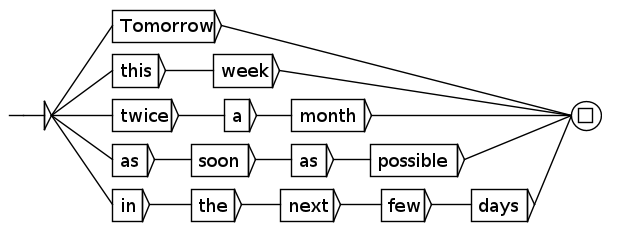
\includegraphics[width=8cm]{resources/img/fig8-6GRFBeautify.png}
		\caption{Automaton with beautify option\label{fig8-6GRFBeautify}}
	\end{minipage}
	\hspace{0.1cm}
\end{figure}
%\begin{figure}[h!]
%	\begin{center}
%		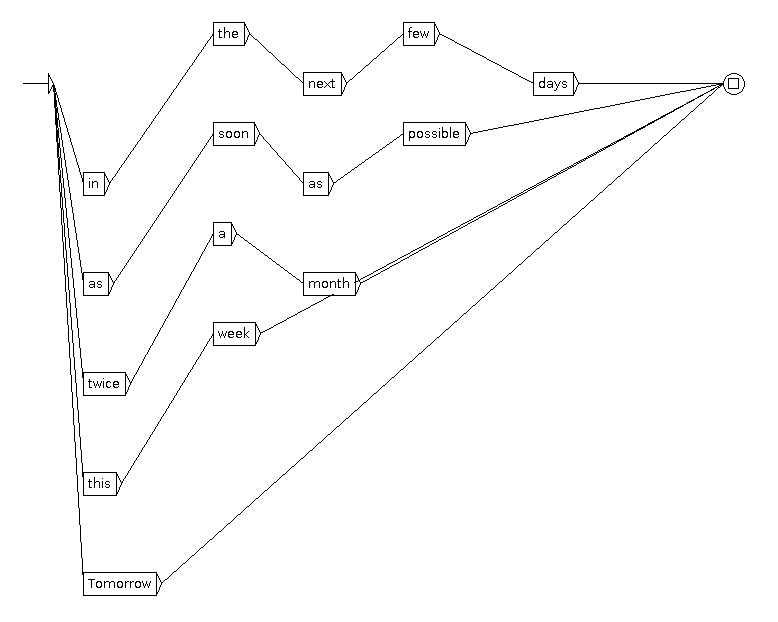
\includegraphics[width=10cm]{resources/img/fig8-5GRFnoBeautify.png}
%		\caption{Automaton without beautify option\label{fig8-5GRFnoBeautify}}
%	\end{center}
%\end{figure}
%\medskip
%\newline
%The graph in figure ~\ref{fig8-6GRFBeautify} was produced without wildcards but with the beautify option activated.
%\begin{figure}[h!]
%	\begin{center}
%		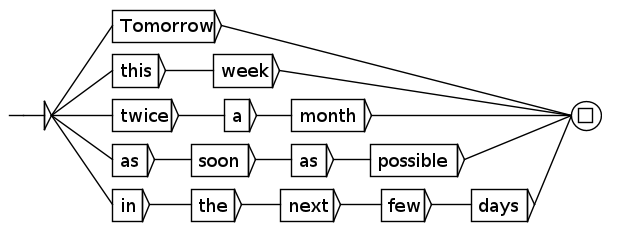
\includegraphics[width=10cm]{resources/img/fig8-6GRFBeautify.png}
%		\caption{Automaton without beautify option\label{fig8-6GRFBeautify}}
%	\end{center}
%\end{figure}
\pagebreak
%%%%%%%%%%%%%%%%%%%%%%%%%%%%%%%%%%%%%%%%%%%%%%%%%%%%%%%%%%%%%%%%%%%%%%%%%%%
\section{Search by approximation} 
\label{approximation}

When you perform a locate operation on a text using a graph produced with the Seq2Grf program, you will find in the match occurences only sequences present in the original sequence corpus.
Some sequences close to those of the sequence corpus might appear in the text and be ignored because they are not in the sequence corpus. 
These sequences should be included in the sequence automaton.
In order to find these sequences,you can produce a graph that recognize all the sequences from the sequence corpus, plus derived sequences that are the result of the application of three kind of wildcards.
Each wildcard makes it possible to apply an operation to generate new sequences.

\begin{itemize}
	\item insertion : for each sequence, add to the automaton all the sequences where <TOKEN> was inserted between two words of the original sequence.
	\item replacement : for each sequence, add to the automaton all the sequences where i tokens have been replace by <TOKEN>
	\item deletion : for each sequence, add to the automaton all the sequences where a token has been deleted
\end{itemize}
Each of these operations can be applied several times to the original sequences.
Applying this grammar to a text will introduce approximations in the search of the sequences in the text.

When wildcards are used, the produced graphs follow these rules :
\begin{itemize}
	\item both original and derived sequences are included in the automaton
	\item no empty sequence nor sequence made only with wildcards will be added to this graph (such sequences could be produced by deletions or replacements on short sequences)
	\item no insertion of a wildcard at the head or tail of a sequence
	\item every token of a sequence including the first and last can be replaced by a wildcard
\end{itemize}
The graphs produced using wildcard contain many erroneous sequences and must be confronted with corpora by a locate to keep only the relevant sequences. These sequences might be used to produce a new graph you might want to keep.

\bigskip

The graph in figure ~\ref{fig8-7GRF1replace} was produced with replacement of 1 token and with the beautify option activated.
\begin{figure}[h!]
	\begin{center}
		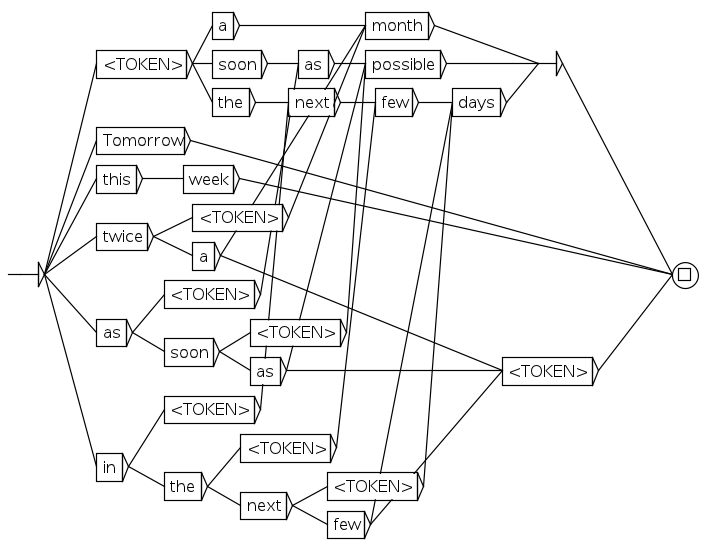
\includegraphics[width=8cm]{resources/img/fig8-7GRF1replace.png}
		\caption{Automaton with one replacement allowed\label{fig8-7GRF1replace}}
	\end{center}
\end{figure}
%\bigskip
%\bigskip
%\noindent 
%You can see here an example with one insertion allowed : 
%\begin{figure}[!ht]
%\begin{center}
%\includegraphics[width=10cm]{resources/img/fig7-seq2grf4.png}
%\caption{Automaton with one insertion allowed\label{fig7-seq2grf4}}
%\end{center}
%\end{figure}&